\documentclass[11pt,a4paper]{article}

\usepackage[margin=2.4cm]{geometry}
\usepackage[T1]{fontenc}
\usepackage{lmodern}
\usepackage{amsmath}
\usepackage{graphicx}
\usepackage{booktabs}
\usepackage{xcolor}
\usepackage{float}
\usepackage[font=small,labelfont=bf]{caption}
\usepackage{subcaption}
\usepackage[hidelinks]{hyperref}

\graphicspath{{figures/}}
\setlength{\parskip}{4pt}
\setlength{\parindent}{0pt}


\title{\textbf{Longevity Risk in a Dutch Pension Portfolio}\\[2pt]
\large Mortality projection, liability valuation and stress testing}
\author{Daniel Wolff}
\date{Valuation date: 30 September 2026}

\begin{document}
\maketitle

\begin{abstract}
\noindent
This project values the pension liabilities of a synthetic Dutch pension fund with 100{,}000
participants and measures how sensitive that value is to longevity and interest rate risk.
Mortality is projected with a Lee-Carter model fitted to Dutch data from the Human Mortality
Database (R), liabilities are valued with the EIOPA risk-free curve (Python), and the
calculation is independently rebuilt and reconciled in Excel. The best-estimate liability (BEL)
is EUR 12.3 bn with a duration of 14.5 years. Across 1{,}000 simulated mortality scenarios, the
99.5\% quantile of the BEL lies EUR 583 mln (4.8\%) above the central estimate, compared with
EUR 959 mln (7.8\%) under the Solvency II standard-formula longevity shock. A 1\% fall in
interest rates raises the BEL by 15.9\%, making interest rate risk roughly twice as large as
longevity risk.
\end{abstract}

\section{Introduction}

A pension fund promises lifelong payments. Two things determine how much money it needs today
to keep that promise: how long its participants will live, and the interest rate at which future
payments are discounted. Both are uncertain. If people live longer than expected, payments
continue for more years; if interest rates fall, every future payment becomes more expensive
in today's money.

This report answers three questions for a synthetic Dutch fund:
\begin{enumerate}
  \item What is the best-estimate value of the fund's pension liabilities?
  \item How uncertain is that value because of future mortality improvement, and how does a
        model-based measure compare with the Solvency II standard-formula shock?
  \item How large is longevity risk relative to interest rate risk, and how does this differ
        between participants?
\end{enumerate}

The work is split over three tools, each doing what it is typically used for in practice:
R for mortality modelling, Python for the liability engine, and Excel for an independent,
reviewable rebuild of the calculation.

\section{Data}

\textbf{Mortality.} Deaths and exposures by single year of age, calendar year and sex for the
Netherlands were taken from the Human Mortality Database (HMD). The models are fitted on ages
30--100 and years 1990--2023, separately for men and women. Figure~\ref{fig:logrates} shows the
historical log death rates: mortality has fallen at all ages, most clearly between ages 50 and
80, and much less at age 95.

\begin{figure}[htbp]
  \centering
  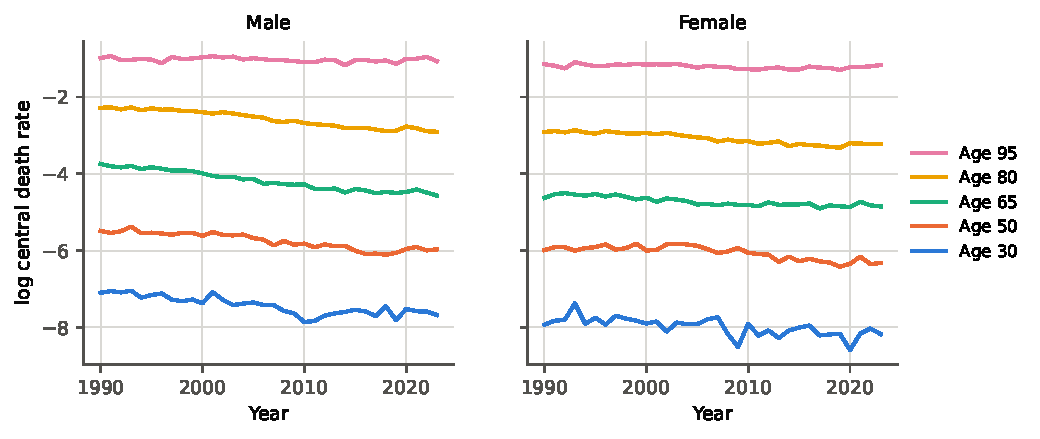
\includegraphics[width=0.9\textwidth]{fig_logrates.pdf}
  \caption{Log central death rates in the Netherlands, 1990--2023 (HMD).}
  \label{fig:logrates}
\end{figure}

\textbf{Interest rates.} Liabilities are discounted with the EIOPA risk-free rate term structure
for the euro of 30 September 2026 (spot rates, no volatility adjustment). The spot rate is about
3.6\% at 10 years and 3.5\% at 30 years, and converges towards the ultimate forward rate
beyond the last liquid point.

\textbf{Portfolio.} The fund is synthetic, generated in Python with a fixed random seed:
\begin{itemize}
  \item 100{,}000 participants, half men and half women;
  \item 70\% active participants aged 30--67, and 30\% retirees aged 68--94;
  \item salaries drawn from a lognormal distribution with a median of EUR 45{,}000;
  \item pension accrual of 1.75\% per year of service on salary above an AOW franchise of
        EUR 18{,}000, with service counted from age 25 up to the current age (actives) or the
        retirement age of 68 (retirees).
\end{itemize}
Only the pension accrued so far is valued, as Dutch funds do. Retirees receive on average
EUR 21{,}900 per year, actives have accrued on average EUR 11{,}900, and the total accrued
annual pension is EUR 1.49 bn.

\section{Mortality model}

\subsection{Lee-Carter versus Renshaw-Haberman}

The Lee-Carter (LC) model describes the log death rate at age $x$ in year $t$ as
\begin{equation}
  \log m_{x,t} = \alpha_x + \beta_x \kappa_t ,
\end{equation}
where $\alpha_x$ is the average age profile, $\kappa_t$ is a single mortality index over time,
and $\beta_x$ is the sensitivity of age $x$ to that index. The model is fitted by maximum
likelihood assuming Poisson-distributed deaths, using the \texttt{StMoMo} package in R.

A first LC fit on ages 20--100 and years 1970--2023 left clear diagonal bands in the residuals
(Figure~\ref{fig:resid1970}). Diagonals follow birth cohorts, so the model misses cohort
effects, for example for generations born around 1915 and 1940.

\begin{figure}[htbp]
  \centering
  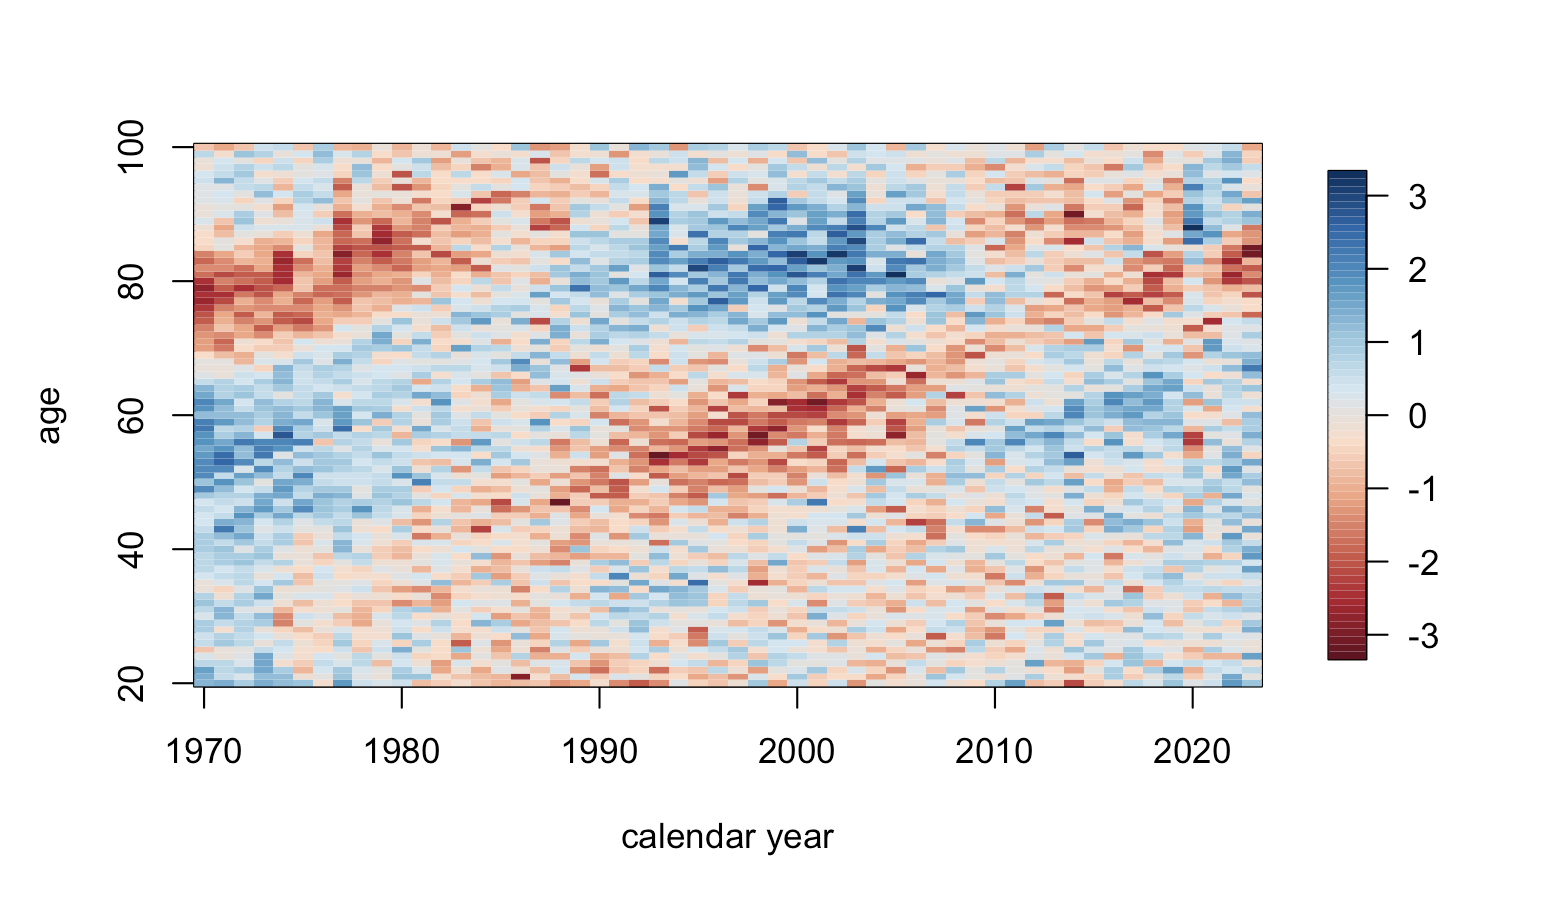
\includegraphics[width=0.5\textwidth]{r_resid_lc_1970.png}
  \caption{Deviance residuals of the first Lee-Carter fit (men, ages 20--100, 1970--2023).
  Diagonal bands indicate cohort effects.}
  \label{fig:resid1970}
\end{figure}

The Renshaw-Haberman (RH) model adds a cohort term $\gamma_{t-x}$ for the year of birth:
\begin{equation}
  \log m_{x,t} = \alpha_x + \beta_x \kappa_t + \gamma_{t-x} .
\end{equation}
RH is known to be hard to estimate. It did not converge on the original data range, and only
converged after restricting the data to ages 30--100 and years 1990--2023. Cohorts with fewer
than three observations were given zero weight, and LC was refitted on exactly the same data
and weights so that both models can be compared fairly.

On this data RH fits clearly better for both sexes (Table~\ref{tab:ic}). Its log-likelihood is
higher, and both AIC and BIC are lower. Since BIC penalises the 97 extra parameters heavily,
the improvement is not just a result of the larger model.

\begin{table}[htbp]
  \centering
  \begin{tabular}{llrrrr}
    \toprule
    Sex & Model & Log-likelihood & Parameters & AIC & BIC \\
    \midrule
    Men   & LC & $-$11{,}518.4 & 174 & 23{,}384.7 & 24{,}391.2 \\
          & RH & $-$10{,}963.9 & 271 & 22{,}469.9 & 24{,}037.3 \\
    \midrule
    Women & LC & $-$11{,}577.5 & 174 & 23{,}503.0 & 24{,}509.4 \\
          & RH & $-$10{,}846.6 & 271 & 22{,}235.2 & 23{,}802.7 \\
    \bottomrule
  \end{tabular}
  \caption{Goodness of fit of Lee-Carter and Renshaw-Haberman (ages 30--100, 1990--2023,
  same weights). Lower AIC and BIC is better.}
  \label{tab:ic}
\end{table}

 The residual heatmaps in
Figure~\ref{fig:resid} confirm this. The remaining structure in the LC residuals, for example around
ages 60--70 in the early 2000s, disappears under RH.

\begin{figure}[htbp]
  \centering
  \begin{subfigure}{0.47\textwidth}
    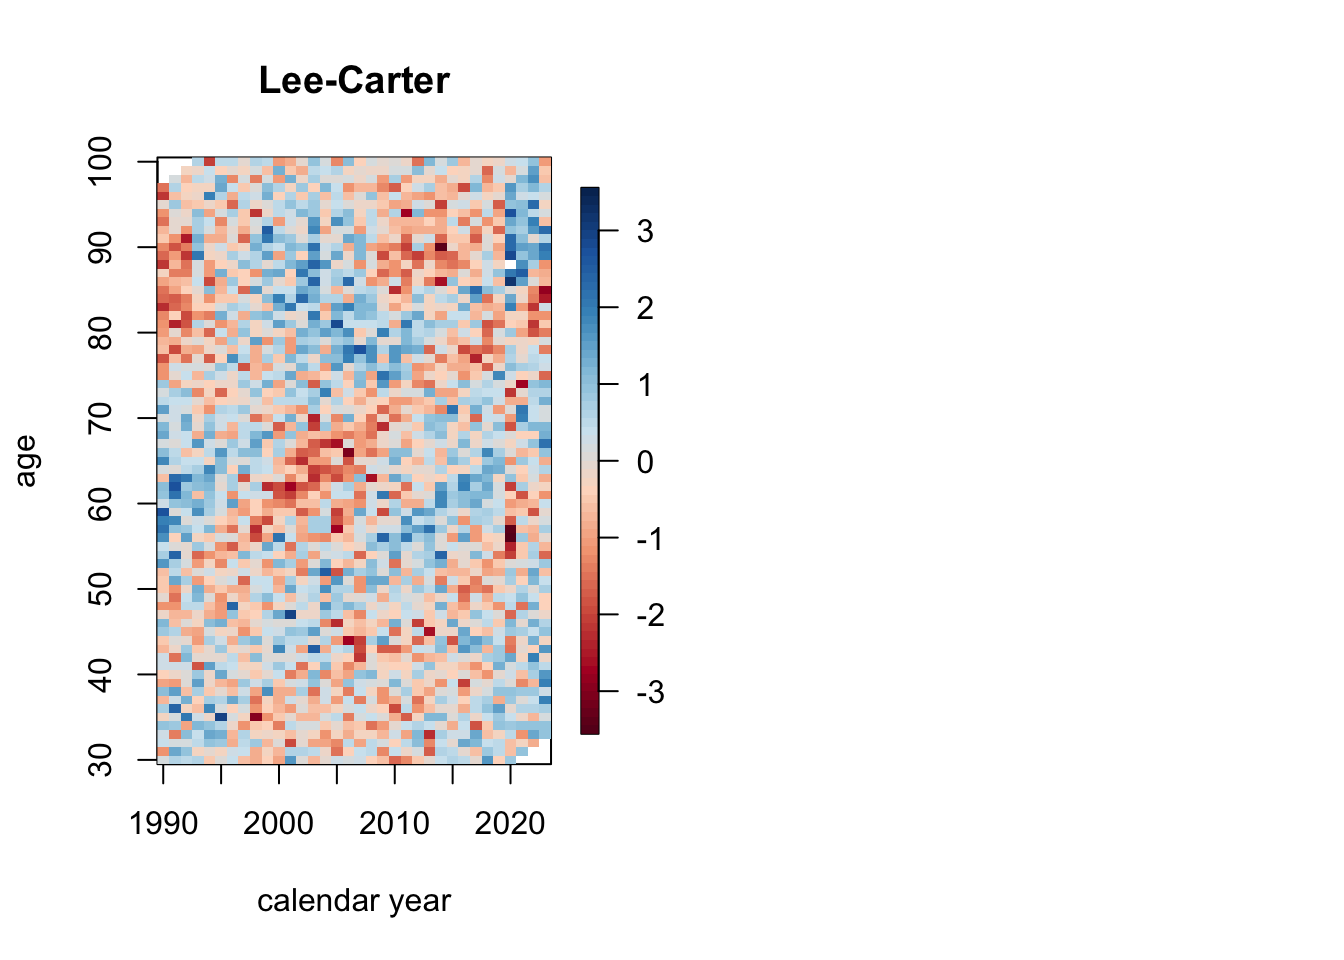
\includegraphics[width=\textwidth]{r_lc_resid_men.png}
  \end{subfigure}\hfill
  \begin{subfigure}{0.47\textwidth}
    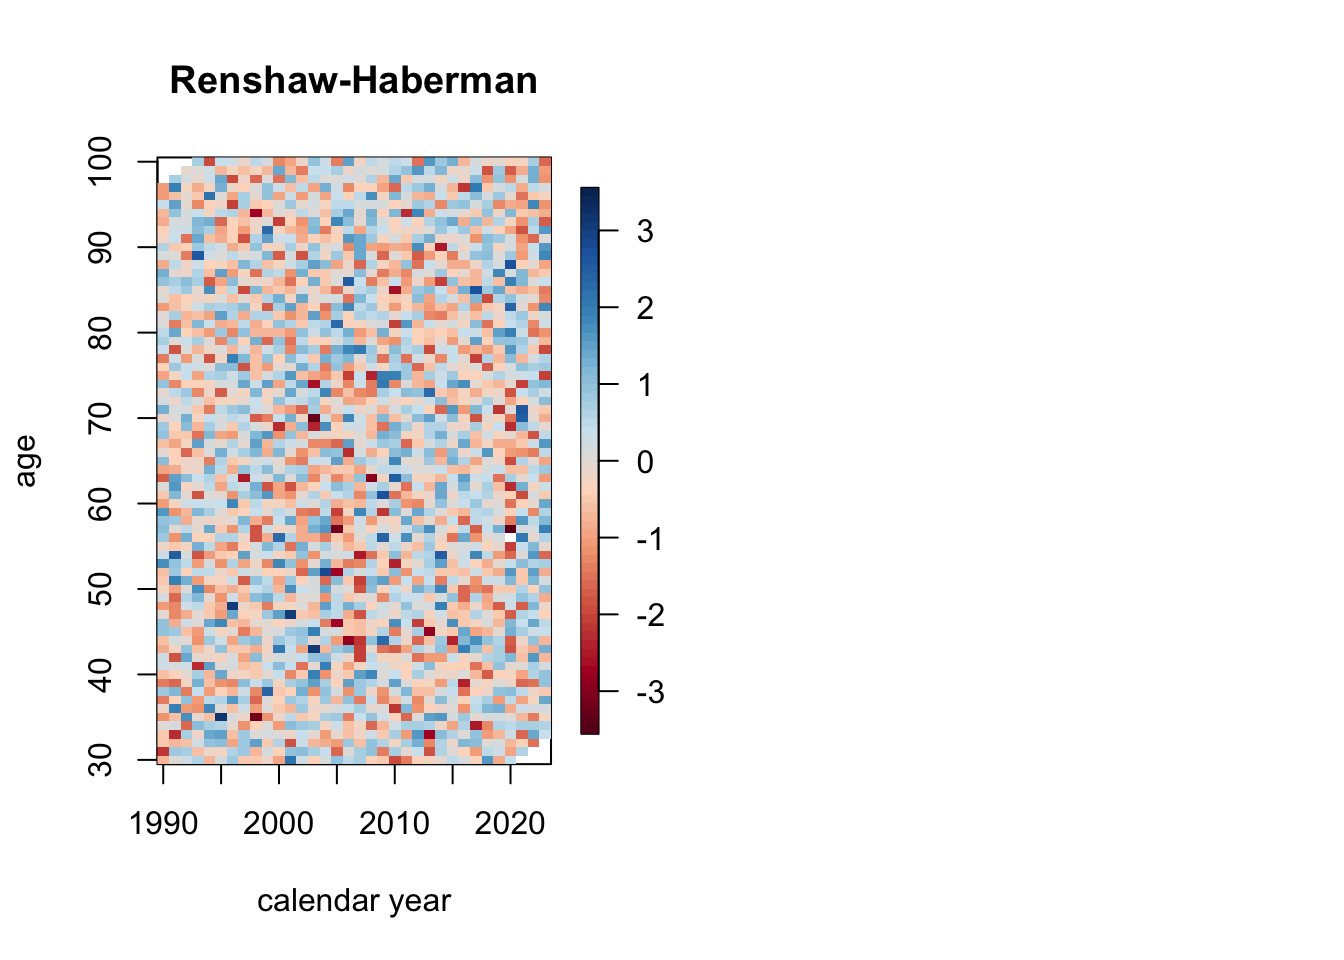
\includegraphics[width=\textwidth]{r_rh_resid_men.png}
  \end{subfigure}
  \caption{Deviance residuals for men, ages 30--100, 1990--2023: Lee-Carter (left) and
  Renshaw-Haberman (right), on the same colour scale.}
  \label{fig:resid}
\end{figure}

\subsection{Forecasting and model choice}

Both models were projected 50 years ahead (2024--2073). For each model, $\kappa_t$ follows a
random walk with drift; for RH, the cohort effect follows an ARIMA(1,1,0) process. For each model,
1{,}000 scenarios were simulated.

A better fit does not guarantee a better forecast. Figure~\ref{fig:e65lcrh} compares projected
period life expectancy at 65. For men, LC projects 21.8 years in 2050 (95\% interval
20.0--23.1). RH projects 26.6 years (24.4--28.6), which implies an improvement of roughly
0.3 years per year, about double what the Netherlands has experienced. For women the pattern
is the same: LC projects 22.6 years in 2050 (20.9--23.9) against 25.2 years (23.6--26.7) for RH.

\begin{figure}[htbp]
  \centering
  \begin{subfigure}{0.49\textwidth}
    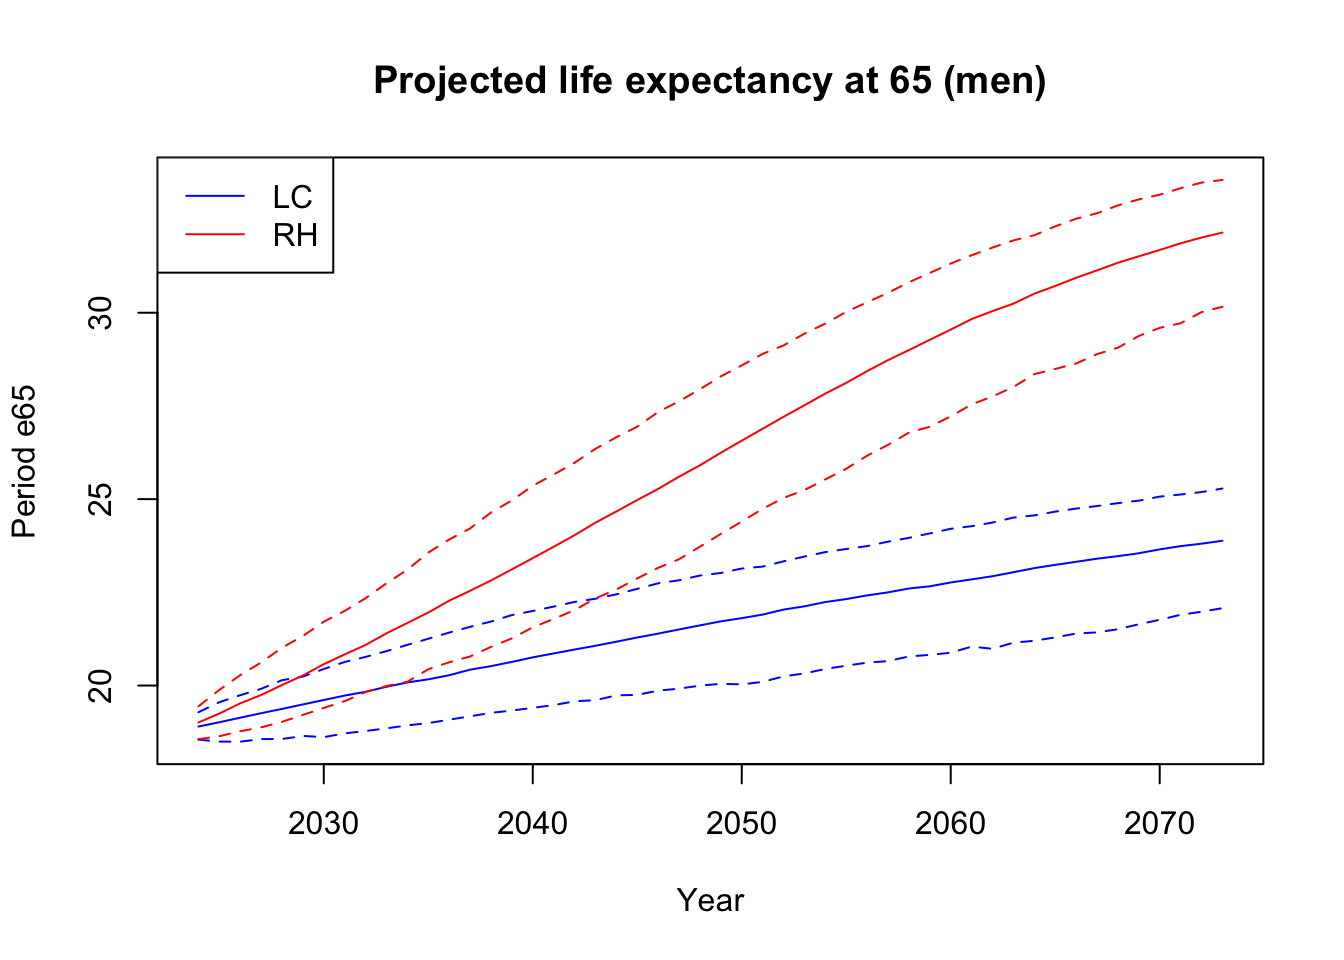
\includegraphics[width=\textwidth]{r_e65_lc_rh_men.png}
  \end{subfigure}\hfill
  \begin{subfigure}{0.49\textwidth}
    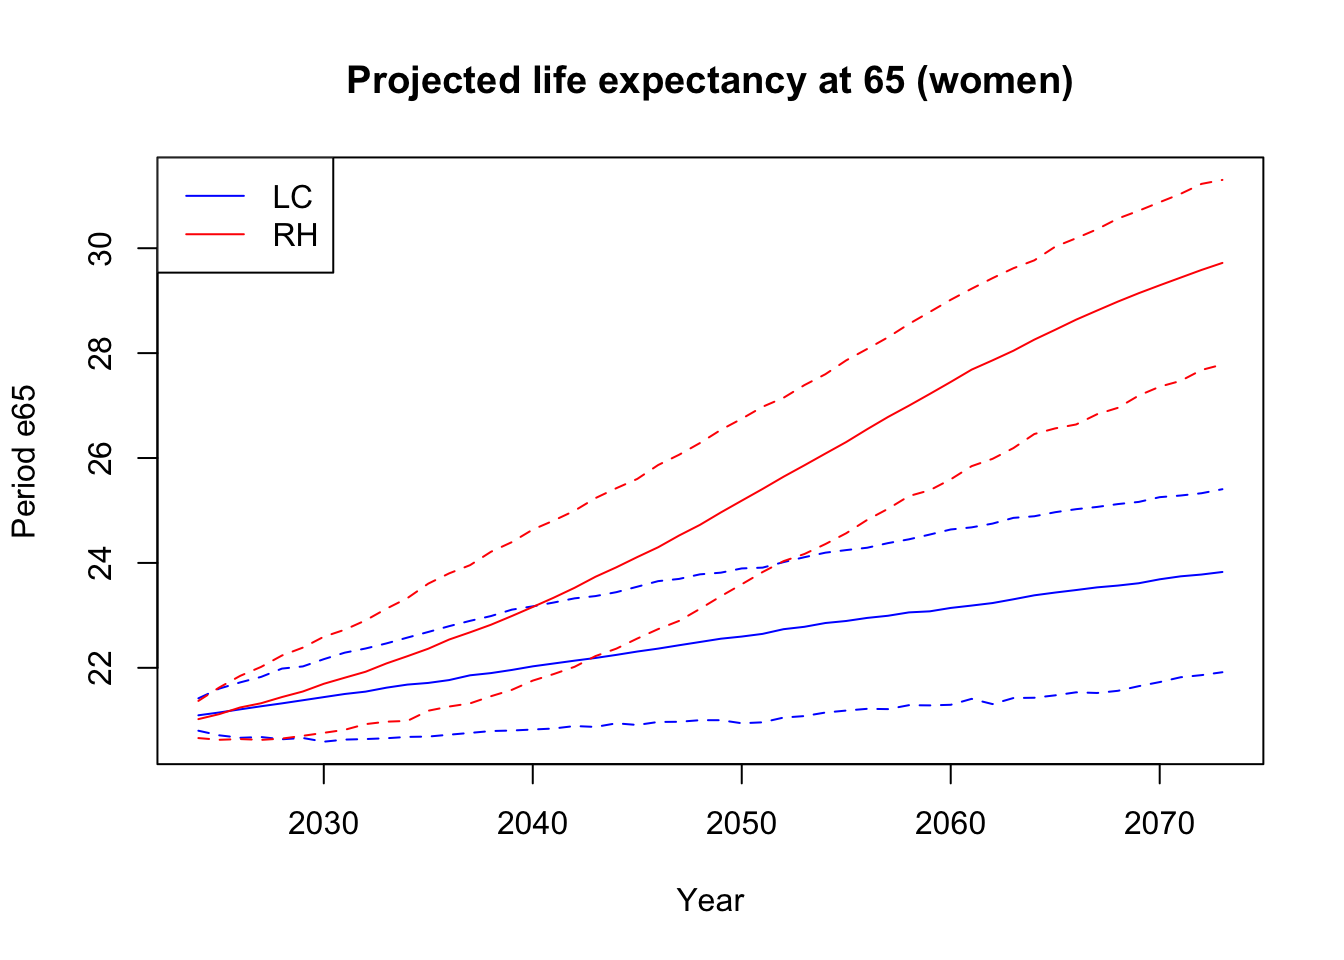
\includegraphics[width=\textwidth]{r_e65_lc_rh_women.png}
  \end{subfigure}
  \caption{Projected period life expectancy at 65 for men (left) and women (right) under
  Lee-Carter (blue) and Renshaw-Haberman (red), with 95\% intervals.}
  \label{fig:e65lcrh}
\end{figure}

The cause is visible in the fitted RH parameters (Figure~\ref{fig:rhparams}). Both $\kappa_t$ and
the cohort effect $\gamma_{t-x}$ are almost perfectly linear, with opposite trends. Within the
data these two trends offset each other, so the fit is good, but they are not separately
identified. When both are extrapolated independently, the offset is lost and the projection
drifts to implausible values. This is a known identifiability issue of RH, which can be solved
with an additional constraint on the cohort trend (Hunt and Villegas, 2015).

\begin{figure}[htbp]
  \centering
  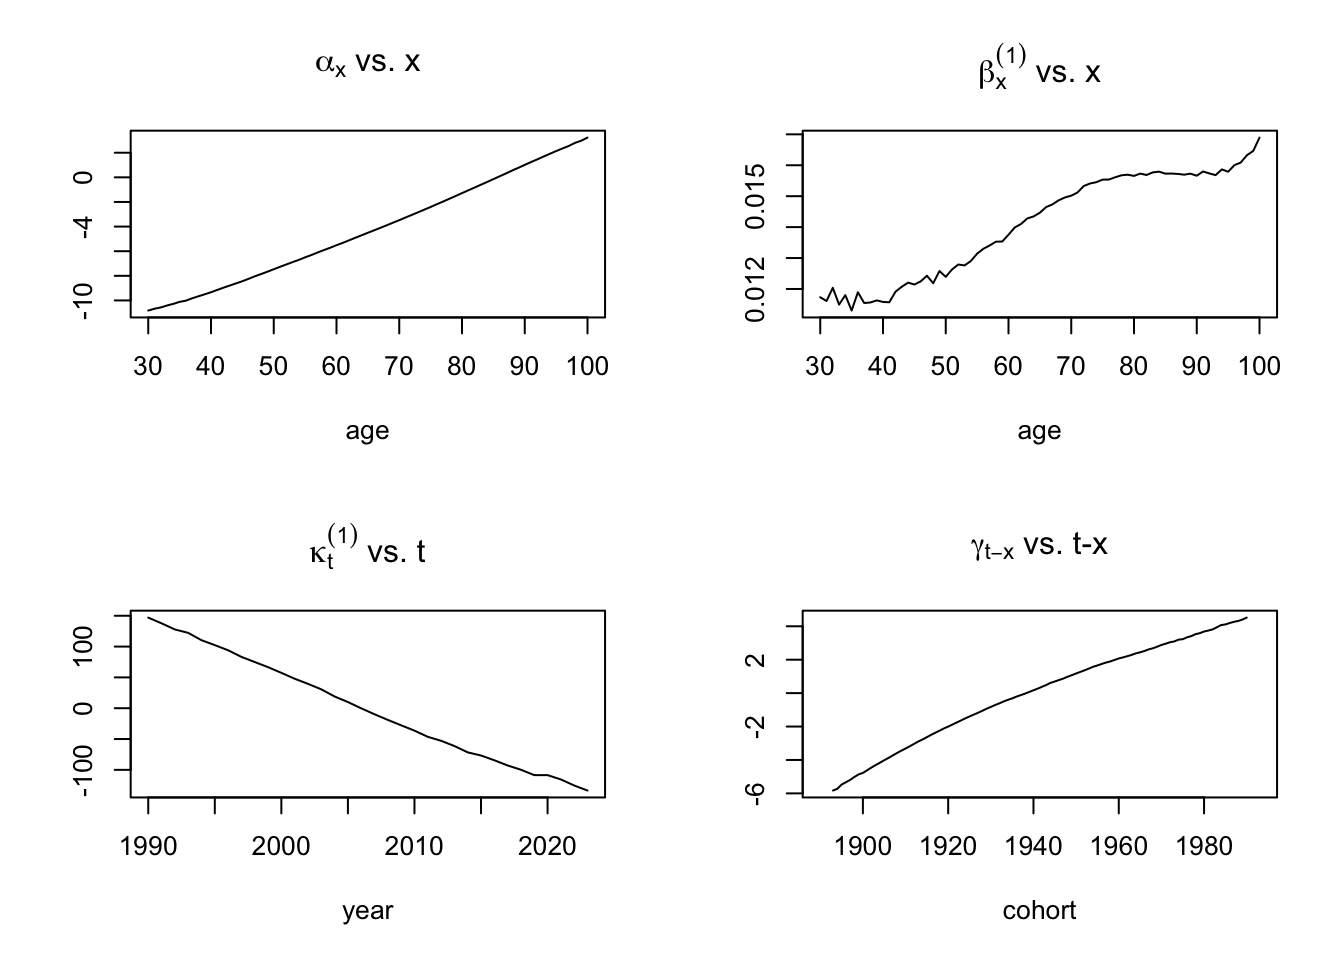
\includegraphics[width=0.6\textwidth]{r_rh_params_men.png}
  \caption{Fitted Renshaw-Haberman parameters for men. Note the near-linear $\kappa_t$ and
  $\gamma_{t-x}$.}
  \label{fig:rhparams}
\end{figure}

\textbf{Decision.} Lee-Carter is used for the valuation. RH is better in-sample, but its
forecasts are not stable enough to base a liability on. The price of this choice is that cohort
effects are ignored, which is listed as a limitation.

\subsection{Lee-Carter projection}

Figure~\ref{fig:e65} shows the LC projection of period life expectancy at 65 for both sexes,
together with the observed history. Life expectancy at 65 rises from 18.8 years (men) and
20.9 years (women) in 2023 to 21.8 and 22.6 years in 2050. The projected gap between men and
women narrows, continuing the trend of the last two decades.

\begin{figure}[htbp]
  \centering
  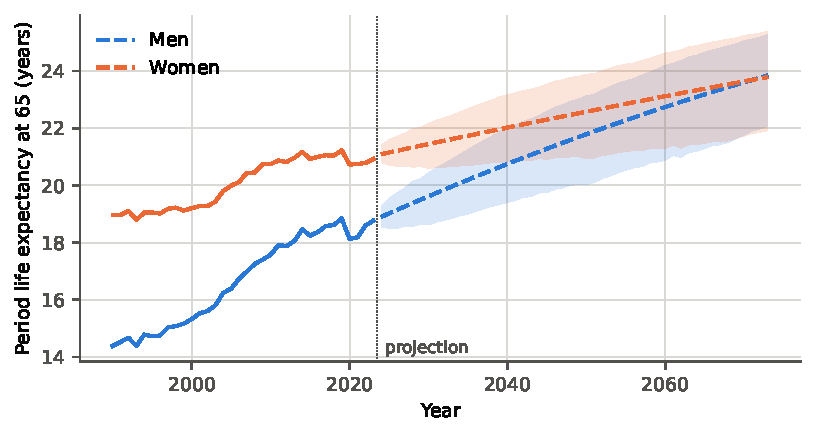
\includegraphics[width=0.7\textwidth]{fig_e65_lc.pdf}
  \caption{Period life expectancy at 65: observed (solid) and Lee-Carter projection
  (dashed) with 95\% interval from 1{,}000 simulations.}
  \label{fig:e65}
\end{figure}

\subsection{Completing the mortality table}

The valuation follows every participant until death, so it needs rates beyond age 100 and beyond
2073. Above age 100, $\log m_x$ is extrapolated linearly in age, using a fit on ages 90--100
for each year and scenario, and the table is closed with $q_{110} = 1$. After 2073 the rates of
the last projection year are kept constant. Death rates are converted to one-year death
probabilities with $q = 1 - e^{-m}$. Figure~\ref{fig:qtail} shows that the completed table
continues smoothly past age 100. It also shows a weakness of LC on this data: because
$\beta_x$ is small at the highest ages, almost no improvement is projected above age 95.

\begin{figure}[htbp]
  \centering
  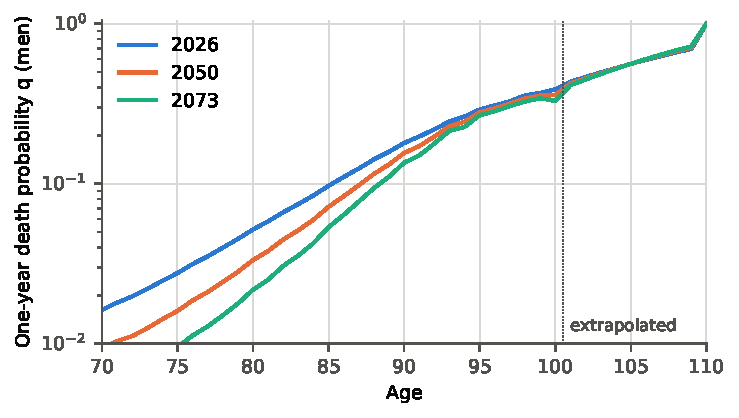
\includegraphics[width=0.6\textwidth]{fig_qtail.pdf}
  \caption{Completed one-year death probabilities for men in 2026, 2050 and 2073.}
  \label{fig:qtail}
\end{figure}

\section{Liability valuation}

\subsection{Method}

Each participant is followed along their generational diagonal: someone aged $x$ in 2026
experiences $q_{x,2026}$ in the first year, $q_{x+1,2027}$ in the second year, and so on. The
probability of still being alive after $t$ years is
\begin{equation}
  {}_tp_x = \prod_{k=0}^{t-1} \left(1 - q_{x+k,\,2026+k}\right), \qquad {}_0p_x = 1 .
\end{equation}
With this table, cohort life expectancy at 65 is 20.5 years for men and 22.0 years for women,
somewhat above the period values because it includes future improvement.

Pensions are paid annually in advance from age 68. The expected cash flow in year $t$ and the
best-estimate liability are
\begin{equation}
  CF_t = \sum_i P_i \; {}_tp_{x_i} \; \mathbf{1}\{x_i + t \ge 68\}, \qquad
  \text{BEL} = \sum_{t \ge 0} CF_t \, (1+r_t)^{-t},
\end{equation}
where $P_i$ is the accrued annual pension of participant $i$ and $r_t$ is the EIOPA spot rate
for maturity $t$. The (Macaulay) duration is the PV-weighted average payment time,
$\sum_t t\,CF_t(1+r_t)^{-t} / \text{BEL}$.

\subsection{Results}

The fund expects to pay EUR 22.3 bn in total. Discounted, this gives a \textbf{BEL of
EUR 12.3 bn} with a \textbf{duration of 14.5 years}. Figure~\ref{fig:cf} shows the expected
payments. They decline from the start, because the current retirees have full pensions while
the actives have accrued only part of theirs. The kink after 38 years marks the retirement of
the youngest actives, after which the fund is in pure run-off.

\begin{figure}[htbp]
  \centering
  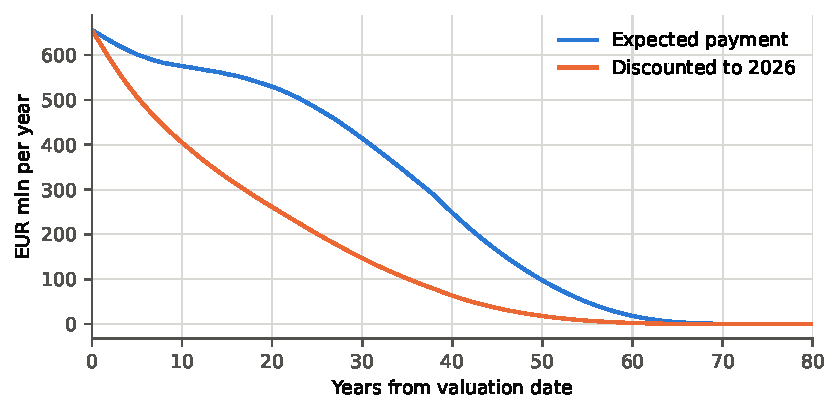
\includegraphics[width=0.7\textwidth]{fig_cashflows.pdf}
  \caption{Expected annual pension payments of the fund, undiscounted and discounted to the
  valuation date.}
  \label{fig:cf}
\end{figure}

\section{Risk analysis}

\subsection{Stochastic BEL}

The full valuation was repeated for each of the 1{,}000 LC mortality scenarios
(Figure~\ref{fig:hist}). The mean of the scenarios (EUR 12.27 bn) is close to the central BEL,
and the standard deviation is EUR 0.27 bn, about 2\% of the BEL. In 90\% of the scenarios the
BEL lies between EUR 11.82 and 12.69 bn. The 99.5\% quantile is EUR 12.86 bn: \textbf{EUR 583 mln
or 4.8\% above the central BEL}. This is the buffer needed to cover longevity trend risk in 199
out of 200 cases, according to this model.

\begin{figure}[htbp]
  \centering
  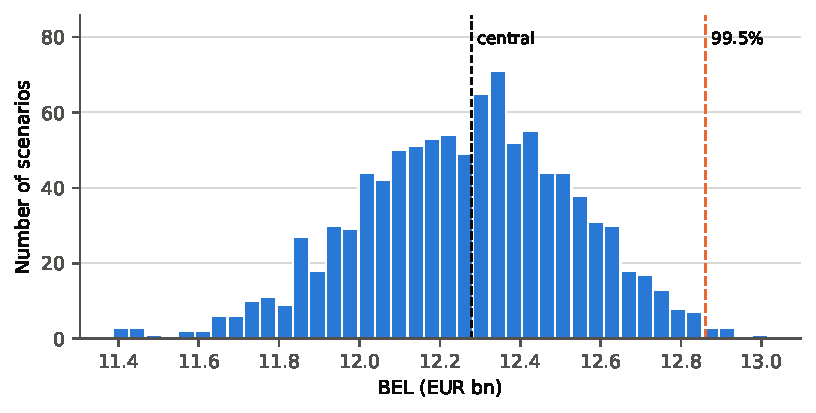
\includegraphics[width=0.7\textwidth]{fig_bel_hist.pdf}
  \caption{Distribution of the BEL over 1{,}000 Lee-Carter mortality scenarios.}
  \label{fig:hist}
\end{figure}

\subsection{Stress tests}

Three deterministic stresses were applied to the central valuation:
\begin{itemize}
  \item \textbf{Longevity:} all mortality rates permanently 20\% lower. This is the longevity shock
        of the Solvency II standard formula.
  \item \textbf{Interest rates $\pm$1\%:} a parallel shift of the whole spot curve. This is a
        simple sensitivity, not the standard-formula interest rate shock, which is
        relative and maturity-dependent.
\end{itemize}

\begin{table}[htbp]
  \centering
  \begin{tabular}{lrrrr}
    \toprule
    Scenario & BEL (EUR bn) & Duration (yrs) & Change (EUR mln) & Change (\%) \\
    \midrule
    Base             & 12.28 & 14.5 &        -- &     -- \\
    Longevity $-$20\% $q$ & 13.24 & 14.9 &   $+$959 &  $+$7.8 \\
    Rates $-$1\%     & 14.23 & 16.0 & $+$1{,}953 & $+$15.9 \\
    Rates $+$1\%     & 10.75 & 13.2 & $-$1{,}528 & $-$12.4 \\
    \bottomrule
  \end{tabular}
  \caption{Fund-level stress tests.}
  \label{tab:stress}
\end{table}

\begin{figure}[htbp]
  \centering
  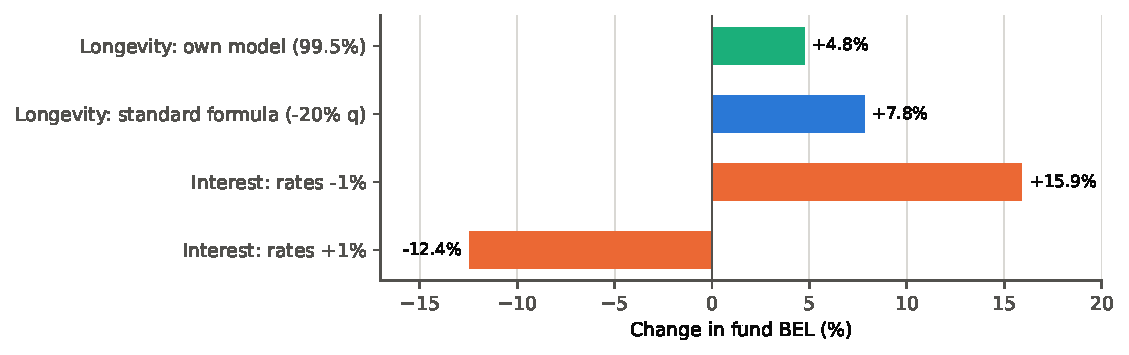
\includegraphics[width=0.92\textwidth]{fig_stress.pdf}
  \caption{Change in fund BEL: model-based longevity buffer, standard-formula longevity shock
  and interest rate sensitivities.}
  \label{fig:stress}
\end{figure}

Three conclusions follow from Table~\ref{tab:stress} and Figure~\ref{fig:stress}:
\begin{itemize}
  \item \textbf{The standard formula is more conservative than the model.} The $-$20\% shock
        requires 7.8\% of BEL, against 4.8\% at the 99.5\% level in the LC model. This is the
        reason insurers develop internal models. Part of the gap is, however, a limitation of
        the model: it only captures the randomness of $\kappa_t$, not parameter or model risk.
  \item \textbf{Interest rate risk dominates.} A 1\% fall in rates costs about twice as much as
        the longevity shock. This is why pension funds and insurers hedge their interest rate
        exposure with long bonds and swaps.
  \item \textbf{The effects are asymmetric.} A fall in rates hurts more ($+$15.9\%) than a rise
        helps ($-$12.4\%), due to convexity. Duration moves as expected: up when people live
        longer, down when rates rise.
\end{itemize}

\section{Excel reconciliation}

To check the Python engine independently, the calculation was rebuilt from scratch in Excel for
10 participants (five actives, five retirees). Python exports each participant's age, pension,
death probabilities along their diagonal and the discount factors. Excel then recomputes
survival probabilities, cash flows, discount factors, BEL and duration with ordinary formulas
and named assumptions. A Data Table runs the calculation for all 10 participants and compares the
result with Python. All 10 BELs agree with Python to within a fraction of a cent, and the cash flows agree in every year.

The Excel model also allows sensitivities per participant (Table~\ref{tab:part}). They show that
the two risks sit in different parts of the fund. The retiree (aged 82) is mainly exposed to
longevity: a lower death rate at high ages adds relatively many expected payments. The active
participant (aged 52) is mainly exposed to interest rates, because their payments only start in
16 years and are therefore discounted over a long period. Combined shocks are larger than the sum of
the separate effects, because the extra years of life are also discounted at the lower rate.

\begin{table}[htbp]
  \centering
  \begin{tabular}{lccc}
    \toprule
    Change in BEL & Longevity $-$20\% $q$ & Rates $-$1\% & Both \\
    \midrule
    Retiree, id 77945 (age 82) & $+$11.7\% & $+$4.3\%  & $+$17.1\% \\
    Active, id 7142 (age 52)   & $+$6.8\%  & $+$28.4\% & $+$37.8\% \\
    \bottomrule
  \end{tabular}
  \caption{Participant sensitivities from the Excel model.}
  \label{tab:part}
\end{table}

\section{From best estimate to required assets}

The BEL is an expected value without any margin. As an illustration of what a Solvency II
insurer would need to hold for this portfolio, using the results above:
\begin{itemize}
  \item \textbf{Risk margin:} the cost of holding capital for non-hedgeable risks until run-off,
        roughly cost-of-capital $\times$ longevity SCR $\times$ duration
        $\approx 6\% \times 0.96 \times 14.5 \approx$ EUR 0.8 bn (about EUR 0.66 bn with the
        4.75\% cost-of-capital rate of the Solvency II review).
  \item \textbf{Solvency capital requirement (SCR):} longevity ($L$) and interest rate risk
        ($I$) are combined with the standard-formula correlation of 0.25 between life and
        market risk, $\text{SCR} \approx \sqrt{L^2 + I^2 + 2 \cdot 0.25 \cdot L I}$.
        Without hedging ($L = 0.96$, $I = 1.95$) this gives EUR 2.4 bn instead of the EUR 2.9 bn
        sum. With a near-perfect interest rate hedge, the SCR is close to the longevity charge of
        about EUR 1.0 bn.
\end{itemize}
In total, the insurer would need about EUR 15.5 bn (126\% of BEL) unhedged, or about
EUR 14.1 bn (115\%) with interest rates hedged, before any additional solvency target. These
figures are rough: the risk margin approximation is simple, the asset side is not modelled, and
the $\pm$1\% shift is not the standard-formula shock. Dutch pension funds fall under the FTK
rather than Solvency II, but the logic of a required buffer on top of the best estimate is the same.

\section{Limitations and next steps}

\begin{itemize}
  \item \textbf{Mortality uncertainty is understated.} Only the random walk of $\kappa_t$ is
        simulated; parameter uncertainty (e.g.\ via bootstrapping) and model risk are not included.
  \item \textbf{No cohort effect.} LC ignores the cohort structure visible in the residuals. A
        constrained RH model (Hunt and Villegas, 2015) could include it with stable forecasts.
  \item \textbf{Little improvement at the oldest ages.} Because $\beta_x$ is small above 95,
        the projection may understate future longevity at high ages; the extrapolation above
        age 100 is a simple log-linear one.
  \item \textbf{Single-population model.} The Dutch AG2024 projection table uses a Li-Lee
        model with a European trend, which gives more stable long-term forecasts. Comparing the
        projection with AG2024 is a natural next step.
  \item \textbf{Run-off versus one-year view.} The 99.5\% quantile covers all future uncertainty
        at once, whereas Solvency II measures a one-year shock.
  \item \textbf{Simplified interest rate risk and no assets.} The $\pm$1\% shift is parallel, and
        hedging is only discussed, not modelled.
  \item \textbf{Synthetic portfolio.} The results describe a stylised fund, not a real one.
\end{itemize}

\section{Conclusion}

The synthetic fund needs EUR 12.3 bn today on a best-estimate basis. Longevity risk adds 4.8\%
at the 99.5\% level according to a Lee-Carter model, well below the 7.8\% implied by the
Solvency II standard-formula shock, while a 1\% fall in interest rates adds 15.9\%. Interest
rate risk is therefore the dominant risk, and the two risks sit in different parts of the fund:
older participants drive longevity risk, younger participants drive interest rate risk. On the
modelling side, the project shows that the best-fitting mortality model is not automatically
the best model for valuation: Renshaw-Haberman fits the Dutch data better than Lee-Carter, but
its forecasts are not stable enough to use.

\section*{References}
\begin{itemize}
  \item Human Mortality Database. University of California, Berkeley (USA), and Max Planck
        Institute for Demographic Research (Germany). \url{www.mortality.org}.
  \item EIOPA, Risk-free interest rate term structures, 30 September 2026.
  \item Lee, R.\,D.\ and Carter, L.\,R.\ (1992). Modeling and forecasting U.S.\ mortality.
        \emph{Journal of the American Statistical Association}, 87(419), 659--671.
  \item Renshaw, A.\,E.\ and Haberman, S.\ (2006). A cohort-based extension to the Lee-Carter
        model for mortality reduction factors. \emph{Insurance: Mathematics and Economics},
        38(3), 556--570.
  \item Hunt, A.\ and Villegas, A.\,M.\ (2015). Robustness and convergence in the
        Lee-Carter model with cohort effects. \emph{Insurance: Mathematics and Economics},
        64, 186--202.
  \item Villegas, A.\,M., Kaishev, V.\,K.\ and Millossovich, P.\ (2018). StMoMo: an R package
        for stochastic mortality modeling. \emph{Journal of Statistical Software}, 84(3).
\end{itemize}

\end{document}
